%! program = pdflatex
 
 \documentclass[12pt]{article}
 \usepackage{geometry} % see geometry.pdf on how to lay out the page. There's lots.
 \usepackage{graphics}
 \usepackage{amsmath}
 \usepackage{fancyvrb}
 \usepackage{gt}
 %\geometry{a4paper} % or letter or a5paper or ... etc
 % \geometry{landscape} % rotated page geometry
 
 % See the ``Article customise'' template for come common customisations
 
 \title{CHILD Users Guide for version R10.7}
 \author{Gregory E. Tucker \and Cooperative Institute for Research in Environmental Sciences (CIRES) \and and Department of Geological Sciences \and University of Colorado, Boulder, CO 80309 USA}
 \date{Last modified: April, 2011} % delete this line to display the current date
 
 %%% BEGIN DOCUMENT
 \begin{document}
 
 \maketitle
 \tableofcontents
 

\section{Overview}
 
The Channel-Hillslope Integrated Landscape Development (CHILD) model is a computer program that simulates the evolution of a landscape. CHILD was created beginning in 1996 and 1997 by Greg Tucker, Stephen Lancaster and Nicole Gasparini, working in Rafael Bras' research group in the Department of Civil and Environmental Engineering at the Massachusetts Institute of Technology. Further development, including creation of many new modules and capabilities, has continued since that time. This guide is written for version R9.4.0, which was released in April 2009.
This guide assumes that you are basically familiar with what CHILD is and what it can do. For basic information about CHILD and its capabilities, see Tucker et al.~(2001a) as well as the references listed in the bibliography at the end of this guide.
 
 \section{Terms of Use}
 
The fine print concerning the use of this software is contained in the GPU2 license agreement, with the following additions and changes:
\begin{enumerate}

\item
You are free to use the software for purposes of research and education. Any resulting publications should cite Tucker et al.~(2001a) and/or other relevant papers by the developers, as appropriate, and should state the code version used.

\item
If you want to modify the code, you have two options. Option 1 is to communicate with one of the developers to ensure that any changes are properly tested and integrated into the main code base. We have a library of standard runs with which to test any modifications, and will be happy to work with you to avoid bugs, conflicts, and so on. The modified source code would then be incorporated into the source-code repository and given an official version number. Option 2, which we do not recommend, is to create a custom-built offshoot on your own. Under this option, you are responsible for babysitting the modified source code and making sure your modifications have not broken anything. If you choose this option, any publications must describe the code as ``a specially modified version of CHILD'' (or words to that effect), and give a disclaimer to the effect that the custom-modified version has not been formally tested or benchmarked (unless you conducted your own benchmarking tests, in which case you should explain these in your publication).

\end{enumerate}
 
\section{Installing and Compiling CHILD}

CHILD was developed in C++ on a Unix platform. As of this writing, we know that it will compile with the g++ on Mac OS X and via the {\em cygwin} Unix shell (www.cygwin.com) on Windows machines. It should also compile with g++ on a Linux platform. We have compiler scripts for a version of Borland's C++ compiler as well as Intel's {\em icpc} compiler, but as far as I know these have not been used in several years and may no longer work.
Once the installation package has been unpacked, there will be a series of sub-folders containing various bits and pieces. The source code lives in the {\em Code} folder. To compile the program on MacOS X, open a terminal window, navigate to the {\em Bin} folder, and enter: 
\scrtxt{\% make -f childir.mk}
The make utility will create an executable file called {\tt child}.
What do you do if you encounter compiler errors at this point? Get hold of someone who has worked with the model before, and/or someone who's good at fidgeting with compilers. If you do run into a compiler problem and then manage to fix it, I would appreciate hearing about the problem and its solution so others do not have to struggle with the same issue.

If you want to use a compiler other than g++, you will need to modify the make files. The file {\tt childir.mk} is a generic, compiler-independent (we hope) file that reads a second make file (using the {\tt include} command), such as {\tt gccmac.mk}, which is designed for g++ on a mac platform. Near the top of the file is a line that looks like
\scrtxt{include gccmac.mk}
This says ``read the contents of the file {\tt gccmac.mk} before proceeding to the next line.'' If, for example, you want to use the compiler-specific make file {\tt icc.mk} instead of {\tt gccmac.mk}, simply change this line to read {\tt include icc.mk}.
 

\section{An Example Run}

\subsection{Starting the Run}

The CHILD release package should come with several example input files to help you get started. These can normally be found in a folder called {\em Examples} in the distribution. One of the examples is an input file called {\tt ridge\_valley\_ex1coarse.in}. As the name suggests, this configures a model run that simulates ridge-valley topography at a fairly coarse resolution. To run this example, create a folder to hold the output and place a copy of {\tt ridge\_valley\_ex1coarse.in} in this folder. Next, either add child to your path or place a copy of it in the same folder. Navigate to this folder. Run the model by entering the following at the command line:
\scrtxt{child ridge\_valley\_ex1coarse.in}
You should see something like the following:

\small
\begin{verbatim}
This is CHILD, version 2.3.0, April 2004 (compiled  Jul 16 2008 14:20:20)

Creating mesh...
In tLNode, reading 'BRPROPORTION1
In tLNode, reading 'BRPROPORTION1
Computing triangulation...elapsed time (time)= 0 s (clock)= 0 s
done.
Creating edge list...done.
Setting up edg pointer...done.
Setting up CCW and CW edges...done.
Setting up triangle connectivity...done.
MakeMeshFromScratchTipper done.
Creating output files...
Warning: `OPTSINVARINFILT' chosen as match for keyword `OPTSINVAR'.
Warning: `OPTSINVAR' is obsolete and is ignored.
 Use `ST_PMEAN' instead.
Creating stream network...
DETACHMENT OPTION: Power law, form 2
SEDIMENT TRANSPORT OPTION: Power-law  transport  formula, form 2
Writing data for time zero...
tOutput::WriteOutput() time=0
Initialization  done.
0
163.769
211.379
235.582
...

\end{verbatim}
\normalsize
This will be followed by a string of numbers that represent the starting time of ``storms'' (periods of random but constant rainfall intensity), until the simulation finishes. (You can safely ignore the warnings about {\tt �OPTSINVAR�}).

\subsection{Output Files}

The run will create a series of output files, each of which begins with the name {\tt ridge\_valley\_ex1coarse} and has an extension that indicates something about what the file contains (for example, the file  {\tt ridge\_valley\_ex1coarse.area} contains the drainage area at each node at each time slice). The format and contents of these files are described further below. To read and plot the contents of these files, we have developed a suite of scripts written in the Matlab language.

\subsection{Plotting Output}

Start Matlab and navigate to the folder containing the output files. Add to your Matlab path the folder containing the CHILD m-files (you can do this with the Matlab path command). At the matlab command prompt ($>>$) enter the following:
\scrtxt{ctrisurf( 'ridge\_valley\_ex1coarse', 26 );}
This will create a shaded surface plot of the terrain at time slice number 26, which corresponds to a simulation time of 500,000 years (halfway through the 1,000,000-year simulation) (Figure~\ref{examplerun1}). In this example run, the output interval is 20,000 years, so that time slice 1 corresponds to time 0, time slice 2 corresponds to time 20,000, and so on. Try experimenting with plotting different times in the simulation.

 \begin{figure}
    \centering
    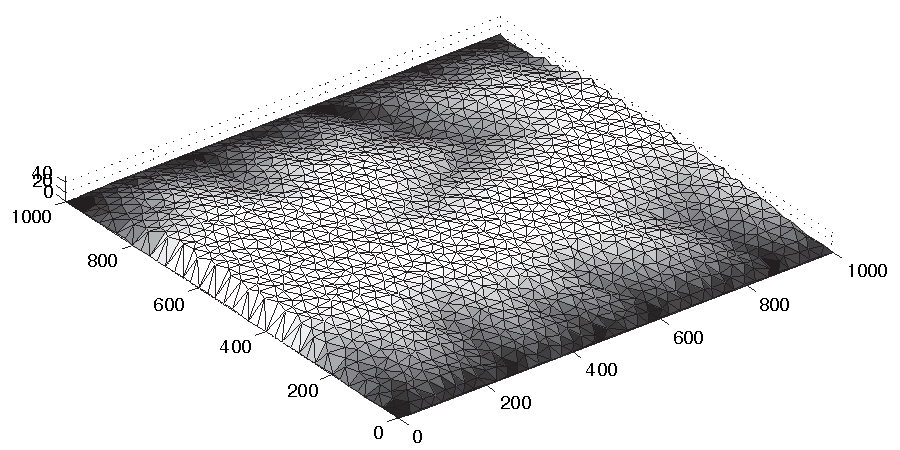
\includegraphics{examplerun1.pdf}
    \caption{Example model run: topographic surface generated by the {\tt ridge\_valley\_ex1coarse} run after 500,000 years of uplift and erosion.}
    \label{examplerun1}
\end{figure}

\section{Configuring an Input File and Starting a Run}

To run a CHILD simulation, you will need to provide an input file (hereafter called the ``main input file'' or simply ``input file'') that contains various required and optional parameters. The main input file can have any name, but by convention main input files normally have the extension {\tt .in}. In most cases, if a simulation mesh is to be generated from scratch, then this is the only file you need.
If you wish to initialize the model from a particular topography, re-start a previous run, several additional files containing information about the initial topography and/or mesh configuration will be needed. These additional files are described below in reference to the various mesh input and/or generation options. (In addition, there are a few special cases that require additional input data in separate files; one example is reading in of a space- and time-varying uplift field).

The command-line syntax for running the model is
\scrtxt{child myinputfile.in [--option]}
where {\tt myinputfile.in} represents the name of the main input file, the format of which is described below, and option represents one or more optionial arguments. For example, the option {\tt --silent-mode} suppresses printing the current time to the screen. To see a list of options, enter {\tt child} with no input file.

The main input file contains a list of process coefficients, option switches, auxiliary file names, and other parameters. Some of these parameters are always required. Many  are optional, and only need to be included when a particular option is selected. Any optional parameters included in the file but not needed in the run are simply ignored. The format for each parameter consists of a line of descriptive text (the ``tag line'') followed by the value of the parameter itself on a second line (the ``value line''). Here is an example of the first part of the example input file {\tt ridge\_valley\_ex1coarse.in}:

\small
\begin{verbatim}
#
# Run control parameters
#
# The following parameters control the name and duration of the run along
# with a couple of other general settings.
# 
OUTFILENAME: name of the run
ridge_valley_ex1coarse
RUNTIME: Duration of run (years)
1000000
OPINTRVL: Output interval (years)
20000
SEED: Random seed used to generate storm sequence & mesh, etc
1
#
# Mesh setup parameters
#
# These parameters control the initial configuration of the mesh. Here you
# specify whether a new or existing mesh is to be used; the geometry and
# resolution of a new mesh (if applicable); the boundary settings; etc.
#
#  Notes:
#
#    OPTREADINPUT - controls the source of the initial mesh setup:
#                    10 = create a new mesh in a rectangular domain
#                    1 = read in existing triangulation (eg, earlier run)
#                    12 = create a new mesh by triangulating a given set
#                        of (x,y,z,b) points in separate file
#    INPUTDATAFILE - use this only if you want to read in an existing
#                    triangulation, either from an earlier run or from
#                    a dataset.
#    INPUTTIME - if reading in a mesh from an earlier run, this specifies
#                    the time to read
#
OPTREADINPUT: 10=new mesh; 1=read existing run/file; 12=read point file
10
INPUTDATAFILE: name of file to read input data from (only if reading mesh)
n/a
POINTFILENAME: name of file containing x,y,z,b data (b=boundary status)
n/a
INPUTTIME: the time which you want data from (needed only if reading mesh)
n/a
OPTINITMESHDENS: no. densifying iterations to initial mesh (0=none)
0
X_GRID_SIZE: "length" of grid, meters
1000
Y_GRID_SIZE: "width" of grid, meters
1000
OPT_PT_PLACE: point placement: 0=uniform, 1=perturbed unif., 2=random
1
GRID_SPACING: mean distance between grid nodes, meters
25
NUM_PTS: for random grid, number of points to place
n/a
TYP_BOUND: open boundary;0=corner,1=side,2= sides,3=4 sides,4=specify
2
OUTLET_X_COORD: x-coordinate of single outlet, if specified
n/a
OUTLET_Y_COORD: y-coordinate of single outlet, if specified
n/a
MEAN_ELEV: mean initial elevation, m
0
RAND_ELEV: max amplitude of random noise appied to initial topography, m
1.0
SLOPED_SURF: Option for sloping initial surface
0
UPPER_BOUND_Z: elevation along upper boundary, m
0
\end{verbatim}
\normalsize
...etc. A hash mark (\#) represents a comment line. These can be used to document the basis for parameter choices and add other notes and reference information. At the start of each tag line is an ``item code'' in capital letters. The correct code for each parameter must be included in order for the model to find and read the parameter  (see below for an alphabetical list of parameters). Parameters can be in any order in the file. In the example above, the first parameter OPTREADINPUT is a required parameter that tells the model whether to create a new (synthetic) mesh, read in an existing mesh (usually generated from a previous run), or create a mesh from an input set of $(x,y,z,b)$ points. In this example, the option for creating a new mesh has been selected. This choice requires several other parameters, including {\tt X\_GRID\_SIZE}, {\tt Y\_GRID\_SIZE}, {\tt OPT\_PT\_PLACE}, and {\tt GRID\_SPACING}. If we had instead chosen to read in an existing mesh, two different optional parameters would need to be included to support this choice: {\tt INPUTDATAFILE}, representing the base name for mesh input files, and {\tt INPUTTIME}, representing the time for which input is read. The sections below describe how to set up a CHILD run with different mesh input/generation options and with different process parameters and options.

\section{Setting Up the Initial Mesh}

CHILD provides several options for generating and/or reading in an initial mesh. You can have the model set up a mesh in any of the following ways:

\begin{itemize}
\item
Generate a new �synthetic� rectangular mesh with a regular hexagonal, perturbed hexagonal, or random arrangement of nodes
\item 
Read in an existing TIN (including a TIN output by another CHILD run)
\item
Generate a mesh from a given set of $(x,y,z,b)$ points
\item
Generate a mesh from a digital elevation grid stored in ArcInfo ascii format (note: as of this writing, this function does not appear to be working properly)

\end{itemize}
The following sections describe how to use these various options.

\subsection{Creating a Mesh from Scratch}
\label{sec:creatingMeshFromScratch}

If desired, CHILD can create a starting mesh with a rectangular domain. Three examples of CHILD-generated starting meshes are shown in Figure~\ref{hexmesh}. Points within the rectangular domain can be regularly spaced in a hexagonal lattice (Figure~\ref{hexmesh}, left), regularly spaced with random offsets in their $(x,y)$ positions (Figure~\ref{hexmesh}, center), or randomly placed within the rectangular domain (Figure~\ref{hexmesh}, right). In the case of a random-offset mesh, the maximum offset amount is equal to $\pm$ 25\% of the nominal point spacing. In all of these cases, there are five possible boundary options (Figure~\ref{boundaries}): (1) a single outlet (open boundary point) in one corner; (2) an open boundary along one side (corresponding to $y=0$); (3) open boundaries along the $y=0$ and $y=y_{max}$ sides; (4) open boundaries along all four sides; and (5) a single outlet point at a specified location. In each case except \#3, the initial elevation is equal to a specified mean elevation plus or minus a random variable (uniformly distributed), the maximum amplitude of which is set by the parameter RAND\_ELEV. In case \#3 (open boundaries on two opposite sides), the elevation of the upper ($y=y_{max}$) boundary is specified ({\tt UPPER\_BOUND\_Z}), and the elevations of the points are set so as to create a uniform gradient between the two boundaries, plus random vertical offsets.

 \begin{figure}
    \centering
    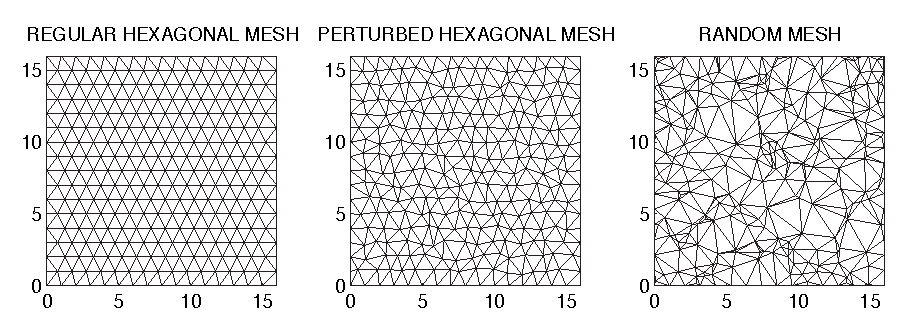
\includegraphics{hexmesh.pdf}
    \caption{Illustration of three different mesh-configuration options.}
    \label{hexmesh}
\end{figure}

 \begin{figure}
    \centering
    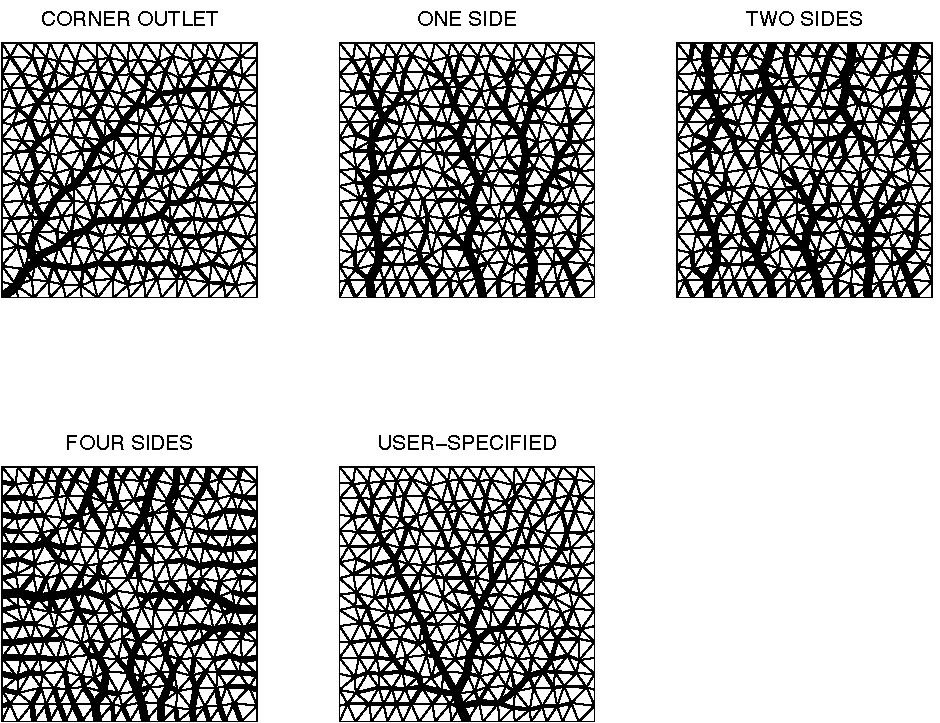
\includegraphics{boundaries.pdf}
    \caption{Illustration of five different boundary-control options.}
    \label{boundaries}
\end{figure}

To start a run with a new rectangular mesh, set \ctag{OPTREADINPUT} to 10. The parameter \ctag{OPT\_PT\_PLACE} controls the type of point placement (0, 1, and 2 for regular, offset, and random, respectively), and the parameter \ctag{TYP\_BOUND} controls the open boundary configuration (0, 1, 2, 3, and 4 for corner, one side, two sides, four sides, and user-specified, respectively). Additional parameters required with these different options are discussed below.

\subsubsection{Setting Up the Configuration of a Synthetic Mesh}

The dimensions of the rectangular mesh are set using the parameters X\_GRID\_SIZE and Y\_GRID\_SIZE (in meters). Set the option for point placement, OPT\_PT\_PLACE, to 0, 1 or 2 for regular, perturbed, or random points, respectively. In the case of regular or perturbed-regular point placement, the mean point spacing (GRID\_SPACING) must be specified. In the case of random point spacing, the total number of interior points, NUM\_PTS, must be given. In any event, the mean elevation (MEAN\_ELEV) and a seed for the random number generator (SEED) must always be provided when a new rectangular mesh is generated.
 
\subsubsection{Boundary Configuration Options}

Set the option TYP\_BOUND to specify the boundary type. For a two-sided boundary, you must also specify the elevation of the upper boundary (which can be different from zero) using the parameter UPPER\_BOUND\_Z. For a user-specified outlet location, give the outlet coordinates in OUTLET\_X\_COORD and OUTLET\_Y\_COORD (note that an outlet cannot be placed in the interior of the mesh).
 

\subsection{Reading in an Existing Mesh}

You can start a CHILD run using an existing triangulation. The triangulation normally comes from a previous CHILD run, but it could also be, for example, a TIN output from a GIS program (however, if you wish to start a run from an existing terrain, it is usually much simpler to have CHILD generate a mesh from a set of $(x,y,z)$ points rather than trying to create a mesh yourself and get it into the right format). The input mesh data format is the same as CHILD's output format (see see Section~\ref{sec:outputfiles}), and consists of four ascii files that contain data on nodes, edges, triangles, and node elevations, respectively. The files must bear the same base name and have the extensions .nodes, .edges, .tri, and .z (as in foo.nodes, foo.edges, foo.tri, foo.z). Each file may contain triangulations for multiple time intervals (obviously in the case of GIS data this does not apply; only one ``time slice'' would be included in the file).

The format of the node file consists of the time represented by the triangulation on the first line, the number of nodes (including boundaries) on the second, and on the subsequent lines the following information for each node: x-coordinate (meters), y-coordinate (meters), ID of one of its connected edges, and a boundary code. (If inputting a mesh that is not the output of a previous run, simply use 0 for the time code). For example:

\small
\begin{verbatim}
 0
289
0.50627 1.134 1424 0
1.02798 1.80433 2 0
0.96638 2.79677 4 0
\end{verbatim}
\normalsize
...etc

The nodes are assumed to be in order by ID number, starting with 0 and ending with $N-1$, where $N$ is the number of nodes. The boundary codes are 0 for an interior point, 1 for a closed boundary, and 2 for an open boundary. {\em Note that points flagged as interior points cannot be on the perimeter of the mesh; an error will occur if any such points exist.}

The format of the other three files is similar in that each time-slice begins with the time value and the number of elements (either edges, nodes, or triangles). In the edge file, each row must contain the ID of the origin node, the ID of the destination node, and the ID of the edge that lies counter-clockwise (relative to the origin). Complementary edge pairs, which are directed edges that share the same endpoints but have opposite orientations, {\em must be together on the list} (for more on the edge-node-triangle data structures, see Tucker et al., 2001b). An example of an edge file is shown below:
 \small
\begin{verbatim}
0
1600
225 0 1417
0 225 34
1 0 30
0 1 1424
\end{verbatim}
\normalsize
...etc. Notice how complementary edge pairs are always grouped together. As with nodes, the edges should be listed in order by ID number.

Each row of the triangle file contains the ID numbers of the three vertex nodes in counter-clockwise order, the ID number of the three triangles opposite these vertex nodes (or -1 if no triangle lies opposite a given face), and the ID numbers of the three clockwise-oriented directed edges. These edges are listed in the same order as their origin vertices, i.e., edges $0\rightarrow 2$, $1\rightarrow 0$, and $2\rightarrow 1$. Triangles are also listed in order by ID.

The node elevations file has the same header format as the others (time followed by number of nodes). The header for each time step is followed by a series of lines that contain the elevation in meters of each node, in order by ID number.

Note: CHILD includes a consistency checking routine to make sure the mesh format is valid, but this is not guaranteed to be foolproof. In particular, the model does not test whether the input triangulation is Delaunay.

\subsection{Creating a Mesh from a Set of Points}
\label{sec:createMeshFromPoints}

CHILD can construct a mesh from an input set of $(x,y,z,b)$ points, where $x$ and $y$ are horizontal coordinates, $z$ is elevation, and $b$ is a boundary code. Such points might be obtained from a field survey, a GIS point coverage, a sampled DEM, etc. To create a mesh from a set of points, set the OPTREADINPUT option to 12. You will then need to specify the name of an ascii file (parameter {\tt POINTFILENAME}) containing the point data. The format for the point data file consists of a header line that gives the number of points, followed by a series of rows that contain the $x$ and $y$ coordinates, the elevation, and a boundary code for each point, as in the following example:
\small
\begin{verbatim}
7
1 3 30 1
3 3 30 1
0 1.5 10 1
2 1.5 10 0
4 1.5 10 1
1 0 0 2
3 0 0 2
\end{verbatim}
\normalsize
The point set in this example is used to construct the seven-node mesh shown in Figure~\ref{pointmesh}. The possible boundary codes are 1 (closed boundary), 2 (open boundary), and 0 (mesh interior). Nodes flagged with boundary code zero must always be within the mesh interior; errors will result if the model encounters an active (0 boundary code) node on the mesh perimeter. In the above example, only one node lies in the mesh interior.
 
  \begin{figure}
    \centering
    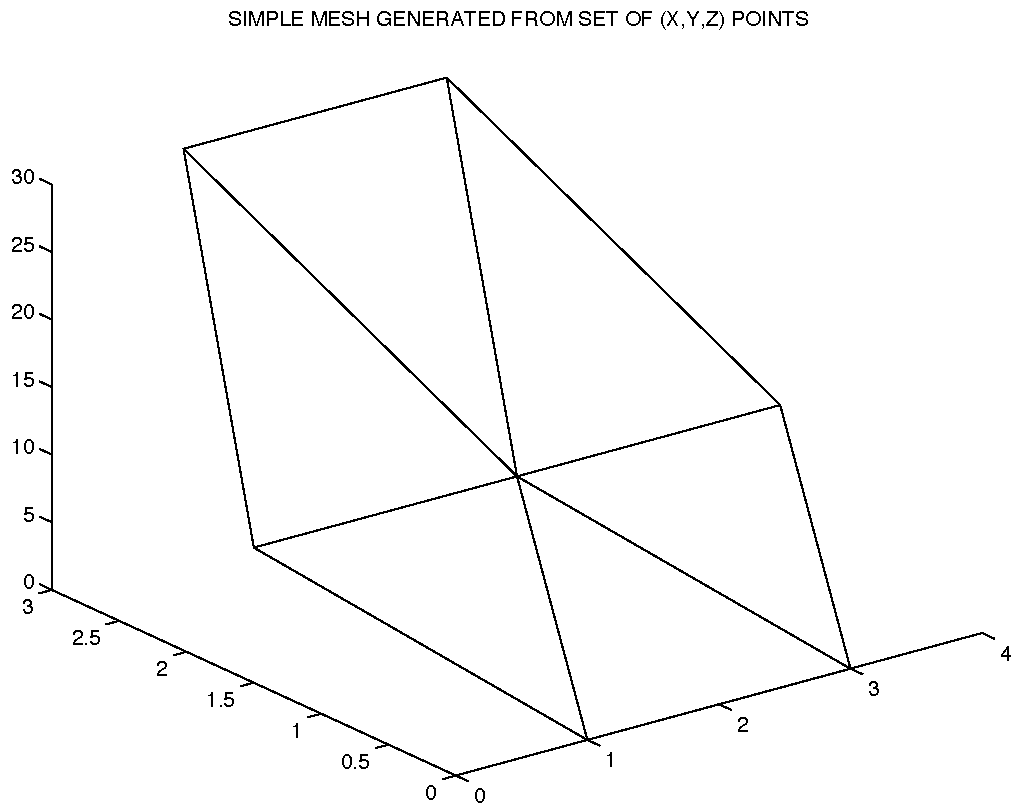
\includegraphics{pointmesh.pdf}
    \caption{A simple mesh generated from a set of seven points.}
    \label{pointmesh}
\end{figure}

\subsection{Generating a Mesh from an ArcInfo Grid DEM}

CHILD can also generate a mesh by interpolating a DEM. The DEM must be in ArcInfo's ascii grid format. In the present version, this capability is somewhat limited. The DEM must describe a single drainage basin, since only one outlet point is created. The resolution of the mesh will be the same as that of the original DEM, and will be uniform in space. The mesh can be either hexagonal, or ``random.'' In the latter case, the mesh starts with one mesh point per DEM point; the $x$ and $y$ coordinates of each point are then offset by a random amount. When a mesh point falls between DEM points, the four-point interpolation procedure of Tetzlaff and Harbaugh (1988) is used to derive the point's elevation. To create a mesh with random offsets from a DEM, set OPTREADINPUT to 3; to create a hexagonal mesh from the DEM, set OPTREADINPUT to 4. Use the parameter ARCGRIDFILENAME to specify the name of the ArcInfo grid ascii file.

\section{Run Control Parameters: Name, Duration, Output, and Options}

Use the OUTFILENAME parameter to specify a base name for the output files. Each output file will have this name followed by an extension that describes the contents of the file. The RUNTIME parameter sets the total duration of the run in years, and the parameter OPINTRVL specifies how often output should be written (also in years).

In addition to data written every OPINTRVL years, if the stochastic climate option (OPTVAR) is used, CHILD also records the intensity, duration, and inter-storm duration for every storm generated, in a file with the extension {\tt .storm}. For each storm, the total volume of material in the landscape at each storm is recorded in a file with extension {\tt .vols}. Using these two files, one can generate a high-resolution plot of the mean elevation of the landscape as a function of time (the script {\em cvolplot.m} does this). For an example, see Collins et al.~(2004). Often, one wants to be able to plot erosion rates at high resolution as well, and for this reason there is a third file, with extention {\tt .dvols}, that records the difference in landscape volume between successive storms.


\section{Climate Parameters}

The parameters ST\_PMEAN, ST\_STDUR, and ST\_ISTDUR set the mean storm intensity, duration, and interstorm interval, respectively (in units of meters and years). To generate a sequence of random storms based on these parameters, set OPTVAR to 1; otherwise, each storm will have the mean values. The stochastic storm-generation model is described by Tucker and Bras (2000), and some of its consequences for landscape evolution are discussed in that paper and by Tucker (2004) and Collins et al.~(2004). The random number generator is initialized by the SEED parameter, so if you want to compare solutions with the same mean values but different random number sequences, simply change SEED (the particular value has no significance).

Note that you can configure a run to operate as a continuous (constant-climate) model by simply turning off climate variation (OPTVAR=0) and, if desired, setting the interstorm interval to zero, in which case ST\_STDUR effectively becomes the global time step. Note also that for long simulations, it is usually convenient to accelerate performance by magnifying the mean storm and interstorm intervals. This preserves the distribution of event sizes while enhancing performance. However, use this approach with caution, since some parameters (such as soil storage capacity) depend on storm duration and would therefore need to be adjusted accordingly.

If desired, any or all of the three storm parameters can be made to vary through time. Implementing time series parameters is described in Section~\ref{sec:timeseries} below.

\section{Runoff Generation and Flow Routing}

The FLOWGEN parameter controls the model�s runoff generation options. Possible values are:

\begin{enumerate}
\item
Uniform Hortonian (infiltration-excess) runoff
\item
Saturation-excess runoff using the O'Loughlin (1986) method
\item
Saturation-excess runoff using the modified Beven and Kirkby (1979) method
\item
Uniform soil-storage capacity (``bucket'' model)
\end{enumerate}
The physics and math behind each of these are summarized in Tucker et al.~(2001a). The Hortonian runoff option is the simplest. It represents a space-time constant soil infiltration capacity, and requires two additional parameters: the soil infiltration capacity (INFILTRATION) in meters per year, and an option for sinusoidal time-variation in infiltration capacity (OPTSINVARINFILT). The latter option causes infiltration capacity to vary sinusoidally in time, with period PERIOD\_INFILT and maximum value MAXICMEAN.

The uniform storage capacity option also requires the INFILTRATION and OPT-
SINVARINFILT parameters, along with the parameter SOILSTORE, which represents the soil water-storage capacity in meters. The O'Loughlin saturation-excess model requires only a single parameter, the soil transmissivity (TRANSMISSIVITY) in square meters per year. The modified Beven-Kirkby saturation-excess model requires three parameters: the infiltration capacity (INFILTRATION), the infiltration variation option (OPTSINVARINFILT), and a unit soil deficit parameter (TRANSMISSIVITY). (Note that the Beven-Kirkby option uses the TRANSMISSIVITY parameter not as a transmissivity {\em sensu strictu}, but rather as a moisture deficit scaling parameter with units of meters.)

\subsection{Lakes and Sinks}

The CHILD model includes an algorithm to identify and route drainage through depressions in the terrain. The algorithm is described in Tucker et al.~(2001b). To invoke this option set LAKEFILL to 1. Otherwise, water will be assumed to evaporate within sink points.

\subsection{Adding an Inlet}

An ``inlet'' is a point source of water and sediment that represents a through-flowing stream. The inlet option makes it possible to configure simulations that represent a segment of a valley or floodplain, or (as a larger-scale example) a large antecedent river crossing mountainous terrain. To activate an inlet, set OPTINLET to 1. The inlet location must then be specified with INLET\_X and INLET\_Y (with the coordinates given in meters). INDRAREA sets the drainage area at the inlet point (in m$^2$). The volumetric sediment load of each grain size is specified in the parameters INSEDLOAD1, INSEDLOAD2, etc.\ (one for each grain size fraction).


\section{Hydraulic Geometry}

In CHILD, each cell is assumed to contain a channel. The width of that channel is calculated from discharge according to the power-law hydraulic-geometry equations of Leopold and Maddock (1953). The width is used in calculating stress or power at each cell. In addition, depending on the options chosen, CHILD calculates up to three other hydraulic geometry parameters (depth, bed roughness, and bank roughness) using the empirical method of Leopold and Maddock (1953). The width, $W$, depth, $d$, bed roughness, $N$, and bank roughness, $M$, are power law functions of bankfull discharge, $Q_b$, and actual discharge, $Q$, as follows:
\begin{eqnarray}
Q_b = R_b A \\
W_b = k_w Q_b^{\omega_b} \\
{W \over W_b} = {Q \over Q_b}^{\omega_s} \\
d_b = k_d Q_b^{\delta_b} \\
{d \over d_b} = {Q \over Q_b}^{\delta_s} \\
N_{b} = k_N Q_b^{\nu_b} \\
{N \over N_b} = {Q \over Q_b}^{\nu_s} \\
M_{b} = k_M Q_b^{\mu_b} \\
{M \over M_b} = {Q \over Q_b}^{\mu_s}
\end{eqnarray}
where $R_b$ is bankfull runoff rate (m/yr), $A$ is drainage area, and the subscripts $b$ and $s$ refer to bankfull and at-a-station values, respectively. Of particular importance is channel width, because shear stress is calculated on the basis of discharge per unit width. The other three hydraulic geometry variables are used only in special cases.

Parameters relating to hydraulic geometry must always be provided in the input file; their use in the model depends on which process options are used. For simulations that do not use the 
detachment-limited option, channel depth is computed and used as the effective vertical depth over which sediment layers are ``seen'' by flowing water. This will have an influence on erosion and transport only when the material is vertically heterogeneous. 

The stream meander module makes use of all of the hydraulic geometry parameters, and the floodplain deposition module uses bankfull depth and flood depth to compute water surface elevations. Bankfull parameters (width, depth, and roughness) are scaled to a bankfull event size (expressed as an bankfull-event-producing runoff rate in meters per year) which is specified in the parameter BANKFULLEVENT. Additional hydraulic geometry parameters are shown in Table~\ref{tab:hydr}.


\begin{center}
\begin{table}
\caption{Hydraulic geometry parameters.}
  \label{tab:hydr}
 \begin{tabular}{ l c }
   \hline
Parameter key & Symbol \\
   \hline
BANKFULLEVENT & $R_b$ \\
HYDR\_WID\_COEFF\_DS & $k_w$ \\
HYDR\_WID\_EXP\_DS & $\omega_b$ \\
HYDR\_WID\_EXP\_STN & $\omega_s$ \\
HYDR\_DEP\_COEFF\_DS & $k_d$ \\
HYDR\_DEP\_EXP\_DS & $\delta_b$ \\
HYDR\_DEP\_EXP\_STN & $\delta_s$ \\
HYDR\_ROUGH\_COEFF\_DS & $k_N$ \\
HYDR\_ROUGH\_EXP\_DS & $\nu_b$ \\
HYDR\_ROUGH\_EXP\_STN & $\nu_s$ \\
BANK\_ROUGH\_COEFF & $\mu_b$ \\
BANK\_ROUGH\_EXP & $\mu_s$ \\
   \hline
  \end{tabular}
  \label{table1}
 \end{table}
\end{center}

\section{Erosion and Sediment Transport Parameters}

\subsection{Rock and Regolith}

CHILD considers two fundamental types of material: {\em rock} and {\em regolith}. These materials are arranged in a series of one or more {\em layers}. Any cell may have an arbitrary number of layers, and the number and properties of layers may differ from cell to cell. {\em Rock} and {\em regolith} differ in their resistance to detachment (they are described by separate detachment-capacity rate coefficients, as described below), and they may also differ in their grain-size properties (if multiple grain sizes are used). The term ``regolith'' here simply means any relatively loose, unconsolidated sediment (alluvium, colluvium, etc.). Whenever sediment is deposited, it is labeled as regolith. 

By default, a run begins with each cell having a uniform thickness of regolith overlying a rock column of uniform thickness. The thicknesses of these initial regolith and bedrock layers are set by the parameters REGINIT and BEDROCKDEPTH, respectively. BEDROCK depth should be set to a sufficiently large value that the base of the bedrock layer will never be exposed. REGINIT may be set to zero, or it may be set to a very large value, in which case the entire landscape effectively consists of sediment.

\subsection{Overview of Transport, Erosion, and Deposition by Running Water}

The default method for computing transport and erosion by running water works is based on the principle that erosion rate may be limited either by sediment transport capacity or by the flow's capacity to detach bed material. The continuity of mass equation for the time rate of change of height at a cell is

\begin{equation}
{d z_i \over d t} = {1\over \Lambda_i} \left( -Q_{Si} + \displaystyle\sum_{j=1}^{N_i} Q_{Sj} \right)
\end{equation}
where $z_i$ is the surface height at cell $i$, $\Lambda_i$ is the cell's horizontal surface area, $Q_{Si}$ is the volumetric water-borne sediment transport rate out of the cell [L$^3$/T], $Q_{Sj}$ is the transport rate in from neighboring cell $j$, and $N_i$ is the number of neighboring cells that drain to cell $i$ (the summation implicitly includes only those neighboring cells that drain to $i$). CHILD's standard fluvial erosion-transport algorithm calculates $Q_{Si}$ by comparing the potential detachment rate, $D_{ci}$ [L/T], with the potential erosion (or deposition) rate $\phi_i$ [L/T] that would occur if the material consisted of loose, non-cohesive sediment. The latter is equal to the surplus transport capacity divided by the cell area:
\begin{equation}
\phi_i = {1\over \Lambda_i} \left( Q_{Ci} - \displaystyle\sum_{j=1}^{N_i} Q_{Sj} \right)
\end{equation}
The transport rate out of the cell, $Q_{Si}$, is
\begin{equation}
Q_{Si} = 
\begin{cases}
\Lambda_i D_{ci} & \text{if $\phi_i > D_c$} \\
Q_{Ci} & \text{otherwise}
\end{cases}
\end{equation}
If the material is easy to detach ($D_c$ is very large), the transport rate will always be simply equal to the capacity. Conversely, if the material is highly resistant to detachment and/or the transport capacity is always large, the rate of erosion will tend to be limited to the detachment capacity. Cases where $\phi$ is negative represent areas of deposition, in which case detachment capacity is irrelevant.

CHILD also includes two alternative ``global'' algorithms for modeling detachment and transport that were programmed by Nicole Gasparini (the ``undercapacity'' and ``tools'' models; see Gasparini et al., 2007). At the time of this writing, these can only be invoked by changing a hard-coded switch in the source code, and are not discussed further in this guide.

\subsubsection{Detachment-Limited Mode}

Much has been written about the hypothesis that some fluvial systems may be effectively {\em detachment limited}, meaning that sediment supply and transport have relatively little effect on the rate of stream-bed erosion (e.g., Seidl et al., 1992; Howard, 1994; Howard et al., 1994; Whipple and Tucker, 1999; Tucker and Whipple, 2002; Whipple and Tucker, 2002). Detachment-limited behavior will occur naturally where the detachment capacity is small and the transport capacity large (e.g., Tucker and Slingerland, 1994), but it is much more computationally efficient to use CHILD's {\em detachment-limited option}. This invokes an alternative (and faster) solver which assumes that any material eroded by running water is immediately removed from the landscape (it corresponds to ``direct removal'' in the model of Ahnert, 1976). To use this option, set OPTDETACHLIM to 1.

\subsection{Choosing Detachment and Transport Laws}

\subsubsection{Detachment-Capacity Laws}

The DETACHMENT\_LAW parameter determines which detachment-capacity equation will be used. Version R9.4 provides two detachment-capacity laws. Both compute detachment capacity on the basis of bed shear stress, $\tau_0$, which is calculated from discharge, width, and slope:
\begin{equation}
\tau_0 = K_t \left( {Q \over W} \right)^{M_b} S^{N_b}
\end{equation}
where $Q$ is discharge [L$^3$/T], $W$ is channel width, $S$ is gradient from cell $i$ to its downstream neighbor, and $K_t$, $M_b$, and $N_b$ are parameters. These corresponding parameters in the input file are KT (entered in SI units), MB, and NB. Note that although we call $\tau_0$ ``shear stress,'' in fact the parameters could be configured to represent any power-weighted combination of slope and unit discharge. For example, if you wanted $\tau_0$ to represent stream power per unit bed area, you would choose MB = NB = 1 and set KT equal to the unit weight of water.

The two detachment-capacity laws both calculate detachment capacity as a power function of shear stress [sic] over and above a threshold. They differ only in how the exponent is applied; one is based on the common practice of placing the exponent on excess stress, while the other applies the exponent to each term independently, which makes it more tractable analytically (for discussion see Tucker, 2004). The detachment laws and their parameters are:

\begin{description}

\item[DETACHMENT\_LAW=0]
Detachment capacity is computed using:
\begin{equation}
D_c = K_{br} \left( \tau_0 - \tau_c \right)^{P_b}
\end{equation}
where $K_{br}$ is a rate coefficient, $\tau_c$ is a threshold below which no detachment takes place, and $P_b$ is a parameter. 

\item[DETACHMENT\_LAW=1]
Detachment capacity is computed using:
\begin{equation}
D_c = K_{br} \left( {\tau_0}^{P_b} - {\tau_c}^{P_b} \right)
\end{equation}
where the parameters are the same as those above.  

\end{description}
Two different values of $K_{br}$ are specified, one for regolith (parameter KR) and one for bedrock (parameter KB). The units are meters per year per excess ``stress quantity'' in SI units. For example, if you want to explore the commonly used model $D_c = K_{br} ( \tau_0 - \tau_c )$, you would set PB to unity and enter KB and KR in units of meters per year per Pascal of excess stress. The threshold $\tau_c$ is also specified separately for regolith (TAUCR) and bedrock (TAUCB). The threshold values are entered in SI units (for example, in Pascals if PB = 1 or in Watts per square meter if PB = 3/2).

\subsubsection{Transport Capacity Laws}

Version R9.4 provides a menu of seven transport capacity laws from which to choose. Four of these assume a single grain-size fraction, while two distinguish between sand and gravel fractions and a third has an arbitrary number of size fractions. The laws are:

\begin{description}

\item[TRANPORT\_LAW=0: Power law formula, form 1]
This is a power-law shear-stress formula similar to the Meyer-Peter and Mueller equation, with the form:
\begin{equation}
Q_c = K_f W \left( \tau_0 - \tau_c \right)^{P_f}
\end{equation}
The transport efficiency factor $K_f$ is given by the input parameter KF, in cubic meters per second per unit excess stress or stress-related quantity (depending on the value of $P_f$ and the dimensions of $\tau_0$, which as noted above could be configured to represent unit stream power). For example, if $\tau_0$ is treated as a stress and $P_f = 1$, as in the dimensional form of the Meyer-Peter-Mueller equation, then KF has units of $m^2 y^{-1} Pa^{-3/2}$ (of course, the dimensional part of this is made of gravitational acceleration, grain size, and fluid and sediment density). The shear stress is actually calculated separately from the stress used in the detachment capacity law, using the same form but a separate set of exponents:
\begin{equation}
\tau_0 = K_t \left( {Q \over W} \right)^{M_f} S^{N_f}
\end{equation}
It may seem a bit silly to do it this way, but the idea is to allow for maximum flexibility in configuring and exploring different erosion and transport laws.

\item[TRANPORT\_LAW=1: Power law formula, form 2]
This power-law shear-stress formula is nearly identical to the previous one, but with the exponent applied to the stress and threshold terms separately:
\begin{equation}
Q_c = K_f W \left( {\tau_0}^{P_f} - {\tau_c}^{P_f} \right)
\end{equation}
This form departs from the more common practice of putting the exponent outside the parentheses, which as far as I can tell comes from fitting straight lines on log-log plots of data. As Peter Molnar once pointed out to me, there doesn't seem to be any obvious advantage to the former apart from the ease with which it can be pulled off a graph of data, while the latter both makes more sense dimensionally and is more tractable analytically because you can separate the two pieces when you integrate (Tucker, 2004). The parameters and method of calculating $\tau_0$ are the same as in form 1.

\item[TRANPORT\_LAW=2: Bridge-Dominic version of Bagnold formula]
I was introduced to this formula during my first semester in graduate school, in a physical sedimentology course taught by Rudy Slingerland. In retrospect, I'm not sure why he chose to teach (and use) this seemingly little-used bed-load formula, due to Bridge and Dominic (1984), as opposed to a more popular model like Meyer-Peter-Mueller or the original Bagnold(s). I suspect it is because the formula (a) isn't simply a curve fit to data, and (b) has a straightforward derivation from basic principles (see, e.g., Slingerland et al., 1994). At any rate, it was the first bed-load formula I learned, and I have continued to use it over the years partly because, like ``power law form 2,'' it is dimensionally consistent and analytically tractable. The form as implemented by CHILD is
\begin{equation}
Q_c = K_f W \left( \tau_0 - \tau_c \right) \left( \sqrt{\tau_0} - \sqrt{\tau_c} \right)
\end{equation}
where $K_f$ is given by
\begin{equation}
K_f = {a \over \rho^{1/2} (\sigma - \rho ) g \tan \phi }
\end{equation}
where $a / \tan \phi$ is a dimensionless transport-capacity coefficient as discussed by Slingerland et al.~(1994). The input value of KF should include a time-conversion factor from stress in Pascals to sediment flux in cubic meters per year.

\item[TRANPORT\_LAW=3: Wilcock sand-gravel formula]
This is an implementation of a two-fraction (sand and gravel) model developed by Peter Wilcock (1998, 2001). The model and its application in landscape evolution modeling are described in a series of papers by Nicole Gasparini and colleagues (Gasparini et al., 1999, 2004, 2008). To use this model, the number of grain size fractions, NUMGRNSIZE, must be set to 2, and the following additional parameters must be specified: REGPROPORTION1, REGPROPORTION2, BRPROPORTION1, BRPROPORTION2, GRAINDIAM1, GRAINDIAM2.

\item[TRANPORT\_LAW=4: Generic power-law formula for multiple size fractions]
This implements a Meyer-Peter-Mueller-like transport formula with up to nine grain-size fractions. The transport capacity for each size fraction $i$ is:
\begin{equation}
Q_{ci} = f_i K_f W \left( \tau_0 - \tau_{ci} \right)^{P_f}
\end{equation}
where $f_i$ is the proportion of size $i$ on the bed and $\tau_{ci}$ is the effective critical shear stress for the $i$-th size fraction. This transport function option has not been fully tested and should be considered experimental.

\item[TRANPORT\_LAW=5: Willgoose-Riley sand-gravel formula]
This function uses the sediment transport model and parameters in
Willgoose and Riley (1998) to calculate sediment transport rates
of the sand and gravel fraction individually.
For now, this function should only be used with two grain sizes
(it uses the Wilcock model to calculate $\tau_c$)
and it is assumed that grain size one is in the
sand range and grain size 2 is in the gravel range. It should be considered experimental.

\item[TRANPORT\_LAW=6: Simple slope-discharge power law]
This implements the simple transport law:
\begin{equation}
Q_c = K_f Q^{M_f} S^{N_f}
\end{equation}
When using this formula, the output file {\em name}{\tt .tau} contains the transport capacity rather than a shear stress.

\end{description}


\subsection{Soil Creep}

There are two models of soil creep from which to choose: linear and nonlinear. In the linear model, volumetric sediment discharge per unit width, $q_c$, is 
\begin{equation}
\boldsymbol{q}_c = K_d \nabla \cdot z
\end{equation}
where $K_d$ is a transport coefficient with dimensions of [L$^2$/T]. The nonlinear model is the one used by Roering et al.~(1999, 2001):
\begin{equation}
\boldsymbol{q}_c = {K_d \nabla \cdot z \over 1 - \left( \left| \nabla \cdot z \right| / S_c \right)^2 }
\end{equation}
where $S_c$ is a threshold slope gradient at which transport rate tends to infinity. The parameter OPT\_NONLINEAR\_DIFFUSION switches between these two forms. If it is  set to 1, you must also specify $S_c$ through the parameter CRITICAL\_SLOPE. In either case, enter $K_d$ using the tag KD, in square meters per year.

The parameter OPTDIFFDEP, is an option that controls whether diffusive transport contributes to both erosion and deposition, or to erosion only. In some cases, there may be reason to apply diffusion only to convex (erosional) elements of topography, with any deposited sediment assumed to be removed rapidly by water erosion (see, e.g., Moglen and Bras, 1994). Set OPTDIFFDEP to 1 to deactive the deposition component of hillslope diffusion.

\section{Working with Multiple Grain Size Classes}

Three of the sediment-transport models, the Wilcock sand-gravel formula (4), the generic power-law multi-size formula (5), and the Willgoose-Riley sand-gravel formula (6), can handle transport of multiple grain size fractions. The two sand-gravel formulas require two size fractions (sand and gravel). The generic power-law formula is designed to handle an arbitrary number of size-fractions. Note that the number of grain size fractions specified in NUMGRNSIZE must match the transport formula used. It must be 2 for the sand-gravel formulas. It can be any number (within constraints of memory availability and computing speed) for the generic multi-size formula. It must be set to 1 for all other transport formulas. Be careful with this: the model does not check every circumstance to make sure you have done it correctly!

When using multiple grain sizes, you can control the proportion of each size in regolith layers and in bedrock layers (the latter represents the size distribution into which the material erodes). This is done using the parameters REGPROPORTION$i$, for the proportion of size fraction $i$ in regolith layers, and BRPROPORTION$i$, for bedrock layers. A value of each parameter must be set for each size fraction; for example, when using the Wilcock sand-gravel formula, you must specify a value for REGPROPORTION1, REGPROPORTION2, BRPROPORTION1, and BRPROPORTION2. The characteristic diameter of each size fraction is set with the GRAINDIAM$i$ parameters. For more information about the multiple grain-size transport algorithms, see Gasparini et al.\ (1999, 2004, 2008).
 

\section{Working with Stratigraphy}

In general, each model node may include any number of layers of variable thickness and sediment composition. By default, the model initializes with a simple, spatially uniform stratigra-phy that consists of a column of bedrock overlain by a column of regolith. The initial regolith thickness may be zero. The total column thickness must be deeper than the maximum potential erosion depth. The initial thickness of the bedrock and regolith columns are set by the parameters BEDROCKDEPTH and REGINIT, respectively, and their erodibility factors are KB and KR. Alternatively, the model can be initialized with a variable sequence of layers of different thickness, composition, and erodibility at each node. This is the method used to restart a run in which stratigraphy matters, and it simply involves setting the OPTREADLAYER parameter to 1. Layer data are then read from a file having the name specified in INPUTDATAFILE followed by the extension {\tt .lay}{\em i}, where $i$ is the time-slice number. (This file must have the format as the layer output file; typically it is a layer output file from a previous run).

If you want to perform a run with stratigraphy, the procedure as of the current version (summer 2009) is unfortunately rather tedious. (If someone wants to volunteer to implement a new option to read in a specified stratigraphy file, please feel free!) First, you need to do a ``one time step'' run, with the option for layer output switched on (i.e., OPTLAYEROUTPUT=1), and, unless you are reading a previous run, with the layer input switched off (i.e., OPTREADLAYER=0). By ``one time step'' run, I mean a run with an arbitrary small duration (say, 1 year). The output from this run will include a file that has the extension {\tt .lay0}. This is the layer output for time zero, and it is this file that you will modify. The basic procedure is to make a copy of this file, modify it according to your stratigraphic desires, and then save it in the proper layer-file format with a filename that is the same as files from your one-time-step run plus the extension {\tt .lay}. Finally, you create a new input file that re-starts the one-time-step run from time zero, this time with OPTREADLAYER=1. This will cause the model to read your newly modified layer file.

You can use matlab to read, edit, and write the layer file. The script {\tt creadlayers} will read the contents of a layer file. Its usage looks like this:

\small
{\tt [layerdata,nlayers,today]=creadlayers(basenm, ts, numg, format\_version ) }
\normalsize

where {\tt basenm} is the base file name (without extension), {\tt ts} is the time slice number (use 1, which represents time zero), {\tt numg} is the number of grain-size fractions used, and {\tt format\_version} is a flag that should, I think, be normally set to zero. The parameter {\tt nlayers} is a vector whose length equals the number of model nodes, and it stores the number of layers at each node. Most of the data, however, live in {\tt layerdata}, which is an $N\times L \times 4+n_g-1$ matrix: $N$ is the number of nodes, $L$ is the maximum number of layers at a node (a maximum imposed by the matlab script, not CHILD), and $n_g$ is the number of size fractions. The 3rd dimension stores layer thickness, age, exposure time, and a flag indicating whether the material in the layer is categorized as ``bedrock'' or ``alluvium'' (regolith). To modify layer data, you adjust the number of layers, and set the bedrock-alluvium flag (the age and exposure parameters generally are fine to keep at zero; they are just used to track chronostratigraphy and surface exposure, respectively). You also need to create a vector or matrix to represent the detachment-rate coefficient for each layer. I say ``vector or matrix'' because it depends on what you wish to do. If you want erodibility to vary in the horizontal dimension but not the vertical, you simply create a vector for KB values (one for each node) and use the function {\tt cwritelayers} to write the layer info to a file. If you want depth-varying stratigraphy, you'll have to muck about with matlab I'm afraid. You would, I suppose, create a matrix of KB values that is dimensioned $N\times L$ and fill it in with the correct values. Then you need to write the whole thing to a file in the correct format.

Here's an example of the first few lines from a layer file:
\small
\begin{Verbatim}[numbers=left]
 0.00
28323
 2
0.00 0.00 0.00
1.50 10000.000000 1
1.50
0.00 0.00 0.00
10000000.00 0.001 0
10000000.00
 2
0.00 0.00 0.00
1.50 10000.000000 1
1.50
0.00 0.00 0.00
10000000.00 0.001 0
10000000.00
 \end{Verbatim}
 \normalsize
The first line has the time, and the second has the number of {\em interior} nodes (if you want to see what this is, look at the second line of the {\tt .area} file in your one-time-step run). Following this is a record for each node. The record starts with the number of layers at that node. For example, line 3 says that layer 0 has 2 layers. For each layer, if a single grain-size class is used, there are 7 numbers that follow, on three lines. The first line gives layer's creation time, its recent activity time (the most recent time it was influenced by erosion/sedimentation), its exposure time (duration of surface exposure). These are all zeros in the example above. The second line gives the layer's thickness, it's erodibility coefficient ($K_b$ value), and its alluvium-bedrock flag. For example, line 5 says that layer 0 at node 0 is 1.5 meters thick, has a $K_b$ of 10,000, and contains alluvium (regolith). The third line then gives the total thickness in each grain-size class (here, the same as the layer thickness, since there is only one grain-size class). In the example above, layer 1 (beneath layer 0) is enormously thick, has a $K_b$ of 0.001, and consists of bedrock.

Your task is to write a file that contains all of this information in exactly the right format. Alas, a single misplaced number can lead to utter garbage --- but at least it will be obvious, as the model will crash with an error related to layering or possibly to limited memory (e.g., if it mis-reads the thickness as the number of layers and tries to create $10^7$ layers at each node).

May the force be with you. (Sure you don't want to implement that automatic layer input code?)

\section{Tectonics and Baselevel Control}

``Uplift'' here refers to any vertical motion relative to the model boundaries, whether posi-tive or negative. Version R9.4 is a veritable ice-cream shop of uplift functions: there are thirteen from which to choose, in addition to option 0 (which means ``none''). Warning: not all of these have necessarily been tested particularly carefully. The choice of uplift mode is controlled by the parameter UPTYPE. All except option 0 require the parameters UPRATE (rate in meters per year) and UPDUR (duration in years).
\begin{description}
\item[0: None] No baselevel change is applied.
\item[1: Uniform] Uplift of all interior points at rate given by UPRATE.
\item[2: Block] Like 1, but only applied to points where $y>y_\text{fault}$, where $y_\text{fault}$ represents the location of a vertical fault striking parallel to the model's $x$ axis. Requires FAULTPOS.
\item[3: Strike-Slip] Block uplift with strike-slip motion along given $y$ coordinate. Requires SLIPRATE.
\item[4: Propagating fold] Propagating fold modeled w/ simple error function curve. Requires FAULTPOS, FOLDPROPRATE, and FOLDWAVELEN.
\item[5: Cosine warp] 2-D cosine-based uplift-subsidence pattern.
Requires FOLDWAVELEN, TIGHTENINGRATE, ANTICLINEYCOORD, ANTICLINEXCOORD, YFOLDINGSTART, UPSUBRATIO.
\item[6: Block, fault, and foreland sinusoidal fold] Requires FOLDWAVELEN, FOLDLATRATE, FAULTPOS, FOLDUPRATE, FOLDPOSITION.
\item[7: Two-sided differential] Two opposite-side boundaries have different rates of uplift. Requires BLFALL\_UPPER and BLDIVIDINGLINE.
\item[8: Fault-bend fold] Requires SLIPRATE, FAULTPOS, FLATDEPTH, RAMPDIP, KINKDIP, UPPERKINKDIP, and MEAN\_ELEV.
\item[9: Back-tilting normal-fault block] Requires ACCEL\_REL\_UPTIME, VERTICAL\_THROW, FAULT\_PIVOT\_DISTANCE.
\item[10: Uplift rate gradient] Linear gradient in uplift rate in $y$ direction. Requires MINIMUM\_UPRATE, Y\_GRID\_SIZE, and OPT\_INCREASE\_TO\_FRONT.
\item[11: Power-law pattern] Power-law change in uplift rate in the $y$-direction. Requires DECAY\_PARAM\_UPLIFT and Y\_GRID\_SIZE.
\item[12: Uplift rate maps] Reads map(s) of uplift rate from separate file(s). This option allows you to vary the uplift rate in both space and (if desired) time. For any particular period of simulation time, you record the uplift rate pattern in a separate file. This file is called an ``uplift rate map.'' If you want the uplift rate to vary in space but not in time, you only need one uplift rate map. If you want the uplift rates to change over time, you use multiple uplift rate maps. In either case, add the parameter NUMUPLIFTMAPS to the main input file. This tells CHILD how many uplift rate maps to read. 

If you have more than one uplift rate map, you also need to create a separate file to record the starting time for each of the uplift rate maps. This is just an ascii text file with the start time of each map after the first given on a separate line. If you only want one map that starts at time zero, you do not need this file. But if, for example, you want two uplift rate maps, one starting at time zero and one at time 1000, you will create an uplift-map time file that contains only a single line with the number 1000. Tell CHILD the name of this ``uplift time file'' by adding a parameter called UPTIMEFILENAME to the main input file.

Finally, you have to tell CHILD the base name for the uplift rate map files using the parameter UPMAPFILENAME. Each uplift rate map file has this base name followed by a three-digit sequence that indicates the file number. For example, if your UPMAPFILENAME is {\tt myupmap}, and NUMUPLIFTMAPS is 3, then you will need to create three uplift map files named {\tt myupmap001}, {\tt myupmap002}, and {\tt myupmap003}. The format of these text files is simply a list of rates, one on each line, in canonical node order (that is, ordered by x and y coordinates --- the same order as in CHILD's standard output format). One way to create uplift rate maps is to do a very short run that generates a grid. Use the $(x,y)$ coordinates of the grid nodes, as recorded in the {\tt .nodes} file, as the basis for setting the uplift rates on your map(s). Each uplift rate map file should list uplift rates for nodes in exactly the same order that the nodes appear in the {\tt .nodes} file. Note that there is no header for the uplift rate map files---just a list of rates, in meters per year, one on each line.

\item[13: Propagating front] Fault position migrates in $x$ and $y$ directions. Required parameters include FRONT\_PROP\_RATE, UPLIFT\_FRONT\_GRADIENT, and STARTING\_YCOORD.
\item[14: Baselevel fall] The elevation at all open-boundary nodes decreases through time at a rate specifed by the UPRATE parameter.
\end{description}

\section{Parameters that Vary in Time}
\label{sec:timeseries}

Patrick Bogaart, currently of the University of Wageningen in the Netherlands, developed a module called {\em tTimeSeries} that allows parameter values to vary through time in any of several different patterns that you can control. At present, parameters that are implemented as time series parameters include ST\_STDUR, ST\_ISTDUR, ST\_PMEAN, UPRATE, FP\_MU, and FP\_INLET\_ELEVATION. The following section describing how to configure a time series parameter in the input file is taken from the document {\em tTimeSeries class: A short manual} by Patrick Bogaart.

\subsection{How to Create {\em tTimeSeries}-Compatible Parameter Files}

Currently, CHILD uses *.in files to define parameter values. Parameter names
and values are on alternating lines. for example:

\begin{verbatim}
         PARNAME: sample parameter
         3.14
\end{verbatim}
{\em tTimeSeries} uses a similar approach. First of all, it is backward compatible,
thus the example above is also valid if PARNAME is a {\em tTimeSeries} parameter. In
this case the function {\tt par\_ts(time)} in the source code returns 3.14 for every value of {\tt time}.
This behaviour can also be set explicitly:
\begin{verbatim}
         PARNAME: sample parameter
         @constant 3.14
\end{verbatim}
The keyword {\em @constant} is a keyword which tells the TimeSeries system how to
cope with the rest of the string. In this case, it means ``always return a value of
3.14.''

\subsubsection{Wave-Form Parameters}

A more interesting case is of couse a genuine time-variable parameter. Suppose we
want a parameter which behaves as a sine function with mean 2.0, period 100.0
and amplitude 1.5. We then say:
\begin{verbatim}
         PARNAME: sample sine mimicing parameter
         @sinwave 2.0 1.5 100.0 0.0
\end{verbatim}
The general pattern is:
\begin{verbatim}
         PARNAME: comment
         @sinwave <mean> <amplitude> <period> <lag>
\end{verbatim}
where {\tt $<$mean$>$} is the average value of the sine wave, {\tt $<$amplitude$>$} is half the
difference between minimum and maximum values, {\tt $<$period$>$} is the wave period, and {\tt $<$lag$>$} is
the horizontal shift of the wave with respect to a standard sine function. The
standard sine function is thus generated by
\begin{verbatim}
         PARNAME: standard sine wave
         @sinwave 0.0 1.0 6.28 0.0
\end{verbatim}
More specifically, the result which is returned by {\em tTimeSeries} is
\begin{verbatim}
         result = mean + amp*sin((time-lag)*twopi/period);
\end{verbatim}
A variant of the {\em SineWave} function is the {\em BlockWave} function, which operates
exactly like the {\em SineWave} function, except that the wave swaps between
mean-minus-average and mean-plus-average. For example:
\begin{verbatim}
         PARNAME: sample bloc wave
         @BLOCKWAVE 100.0 50.0 1000.0 0.0
\end{verbatim}
results in a value of 150 for the time interval 0-500, and a value of 50 for
the interval 500-1000 and so on.

\subsubsection{Parameter Values Read from a File}

It is also possible to read paramter values from a file, which in its
simplest case is done like this:
\begin{verbatim}
         PARNAME: example showing parameter read from a file.
         @file data.dat
\end{verbatim}
which in combination with the file {\tt data.dat}, having a content like
\begin{verbatim}
         0.0 10.0
         1.0 30.0
         2.0 25.0
\end{verbatim}
generates the following output:
\begin{verbatim}
         10.0, for 0.0 < time < 1.0
         20.0, for 1.0 < time < 2.0
         25.0, for time > 2.0
\end{verbatim}
In general, {\tt time} is assumed to be in the first column of the data file, and the
parameter value in the second column. If this is not the case, then columns can
be set explicitly:
\begin{verbatim}
         PARNAME: example showing parameter read from a file.
         @file data.dat 1 3
\end{verbatim}
reads time from column 1 and parameter values from column 3.

By default, parameter values are not interpolated between time points. A given
parameter is valid until a new time/parameter pair is given. Linear
interpolation is easily obtained by appending the {\tt interpolate} keyword:
\begin{verbatim}
         PARNAME: example showing parameters read from a file.
         @file data.dat 1 3 interpolate
\end{verbatim}
Note that the default behavior can be explicitly set by adding the {\tt forward}
keyword.

An extra option is to indentify time and parameter-value columns by name instead
of column number. If a data file has contents like:
\begin{verbatim}
             %columns: time rainfall
             0.0 10.0
             1.0 30.0
             2.0 25.0
\end{verbatim}
then an entry in the *.in file like
\begin{verbatim}
             PARNAME: example showing parameters read from a file.
             @file data.dat time rainfall interpolate
\end{verbatim}
yields the epected result.
In fact, much more information can be stored within a parameter file. The
following example speaks for itself:
\begin{verbatim}
             %info: This is an example of a data file.
             %This is a comment. it start with an %
             %
             %Now a name=value parameter:
             %pi=3.1415
             %
             %The column names are stored like this:
             %columns:        time    discharge sediment_supply
             %units:          [yr]    [m3/s]          [kg/s]
             %
             %That makes 3 columns. Note the units definition. this is not
             %required
             %
             %now the raw data:
             1970    2145.5      500.1
             1971    2453.2      531.7
             1972    1400.6      481.9
\end{verbatim}
The general pattern of this version of {\em tTimeSeries} definition is thus:
\begin{verbatim}
        @file <filename> <time column id> <par column id> <mode>
\end{verbatim}

\subsubsection{In-Line Parameter Definition}

It seems awkward to introduce a different paramter file for each parameter
whose temporal behaviour is only slighly non-trivial. We can therefore define
the time/parameter value pairs also in the *.in file directly:
\begin{verbatim}
        PARNAME: example showing inline definition
        @inline 1970:2145.5   1971:2453.2    1972:1400.6 interpolate
\end{verbatim}
which implements the same data as in the extended example above. Note that the
colon (:) is used here as a time-value seperator, but a simple space works as
well. It just increases the readability. The general structure of this form
of time series is
\small
\begin{verbatim}
    @inline <time1> <value1> <time2> <value2> ... <timen> <valuen> <mode>
\end{verbatim}
\normalsize
Caveat: lines constructed in this way can be too long for CHILD to handle. The
maximum line length is set in the {\em kMaxNameLength} constant within {\em tInputFile.h}.


\section{Output Files}
\label{sec:outputfiles}
CHILD records information about elevation, slope, drainage area, surface flow directions, surface water discharge, surface sediment composition, shear stress, stratigraphy (``layers''), Voronoi polygon areas, node ID numbers, storm properties, volumes, changes in volume from storm to storm, information needed to re-start random number sequences, and information on the mesh triangulation. Output is written to a series of ascii files at selected intervals beginning with the initial state of the run. Each file generally contains one type of information (e.g., node elevations) and includes output from the start to the end of the run. The format of each file varies somewhat according to the type of data it contains, but most of the output files share the same header format: data for each time-slice is preceded by the simulation time (this line always begins with a space for easy identification) and the number of data elements for the current time-slice (equal to the number of nodes, edges, or triangles, depending on the contents of the file). Following the time come one or more columns of data. The format is illustrated below with a hypothetical node elevation file containing two time slices for a mesh with only three nodes:

\begin{Verbatim}[numbers=left]
 0
3
1.1
2.2
3.3
 100
3
0.1
1.2
2.3
\end{Verbatim}
Lines 1-5 contain data for the first time slice (time = 0 years) and lines 6-10 contain data for the second (time = 100 years). For each time slice, the first value (lines 1 and 6) gives the simulation time, the second value (lines 2 and 7) gives the number of nodes (only three in this case) and the remaining lines give the data (in this case, elevations at nodes 0, 1 and 2).
Note that data elements are always listed in order by ID number, starting from zero. Note also that the number of elements can change between successive time-slices if dynamic remeshing is used. Each output file bears the name specified in the input file (OUTFILENAME) followed by a suffix that indicates something about what the file contains. Output files and their suffixes are listed in Table~2. For more on the data structures used by the triangulation, see Tucker et al.~(2001b).

\begin{table}
\label{tab:outputfile}
\caption{Summary of CHILD output files}
\begin{center}
  \begin{tabular}{ l l }
    \hline
	{\bf File extension} & {\bf Contents} \\
	\hline
	{\tt .area} & Drainage area (m$^2$) \\
	{\tt .dvols} & Change in landscape volume over one storm \\
	{\tt .edges} & IDs of origin and destination nodes, ID of ccw edge \\
	{\tt .inputs} & Record of input parameters \\
	{\tt .lay}{\em i} & Layer information for time slice $i$ \\
	{\tt .net} & ID of downstream neighbor \\
	{\tt .nodes} & Node (x,y) coordinates, ID of one spoke, and boundary code \\
	{\tt .q} & Water discharge at each node (m$^3$/yr) \\
	{\tt .random} & Data for re-starting the random number sequence \\
	{\tt .slp} & Gradient in downstream direction \\
	{\tt .storm} & Inter-storm duration (yr), intensity (m/yr), duration (yr) \\
	{\tt .tau} & Shear stress (Pa) \\
	{\tt .tri} &	 IDs of vertices, neighbor triangles, and edges \\
	{\tt .tx} & Volumetric proportion finest grain size in top layer \\
	{\tt .varea} & Voronoi area of each node (m$^2$) \\
	{\tt .vols} & Landscape volume at each storm \\
	{\tt .z} & Node elevations in meters \\
	\hline
  \end{tabular}
\end{center}
\end{table}

\subsection{Surfer-Compatible Output}

Quintijn Clevis (now at Royal Dutch Shell) developed an option for Surfer-compatible output. If the SURFER option is switched on, the model will generate an ascii output file that can be imported into Surfer for plotting. The file format has the time on the first line and the number of nodes on the second line, followed by one row for each node that contains the $x$, $y$, and $z$ coordinates, the drainage area divided by 10,000, the thickness of the topmost layer, the creation time of the topmost layer, and the recent activity time of the topmost layer. The files are called {\em basename}{\tt .surf}$n$, where {\em basename} is the base name of the run and $n$ is the time slice number, with zero being the starting topography. For example, Surfer-style output for the initial model state in a run called ``frog'' would be recorded in a file called {\tt frog.surf0}.

\section{Error Messages}

Being a research tool, CHILD does relatively little error checking. The burden is on you the user to make sure that the format of your inputs is correct and that the parameter settings are reasonable. However, a limited amount of error handling is provided, and it is common to see error messages when a parameter is missing in the input file, the input mesh contains an error, etc. If you should happen to receive an ``assertion failed'' message, please report it on the Wiki or to Greg Tucker (gtucker@colorado.edu).

\section{FAQ and Common Errors}

\subsection{``Error in Lake Filling algorithm: Unable to find a drainage outlet''}

This error commonly occurs in two circumstances: when you are initializing CHILD from a set of $(x,y,z,b)$ points (see Section~\ref{sec:createMeshFromPoints}), or when CHILD is creating its own mesh with a single water-outlet point (see Section~\ref{sec:creatingMeshFromScratch}). In either case, the the problem arises because there are one or more interior points that are isolated from any open-boundary points. In CHILD, when the Lake Fill algorithm is used, water that rains onto each need must ultimately be able to reach an open boundary node. If, for example, you have an interior node that is surrounded by closed-boundary nodes, the water is trapped and it will generate this error message. Or, if you have a single open-boundary (outlet) node and it is surrounded by closed-boundary nodes, the same problem will occur.

If you are generating a mesh from a user-specified set of points, the easiest way to diagnose the problem is to plot on screen the $(x,y)$ positions of the nodes listed in your points file. Color the points according to their boundary status: for example, blue for interior, red for closed-boundary, and green for open-boundary. Check to see whether the green (open boundary) nodes are all surrounded by red (closed boundary) nodes. Check also for blue nodes that are surrounded by red nodes. Normally, the solution is to edit the boundary status of nodes until you are sure that every blue node can reach a green node without having to cross any red nodes. One thing to watch out for is that blue nodes are not allowed on the mesh perimeter---an error message will result if this occurs.

If CHILD is generating its own mesh with a single outlet, the most practical solution is to nudge the position of the outlet node toward the mesh interior until it gets close enough to connect to one or more of the interior nodes. An alternative solution (which applies only if using a perturbed or random mesh; see Section~\ref{sec:creatingMeshFromScratch}) is to change the value of the random seed parameter ``SEED.'' This will change the positions of the mesh nodes, possibly enough to connect the outlet node to one or more interior nodes. Typically you need to try several different seed values before finding a configuration that works.


\section{Alphabetical List of Parameters}

\begin{description}

\item[ACCEL\_REL\_UPTIME] Uplift option 9: fraction of total time that fault motion has been accelerated.
\item[ANTICLINEXCOORD] (m) Uplift option 5: $x$ coordinate of anticline crest.
\item[ANTICLINEYCOORD] (m) Uplift option 5: $y$ coordinate of anticline crest.
\item[ARCGRIDFILENAME] Name of ascii file in ArcInfo format containing initial DEM.

\item[BANK\_ROUGH\_COEFF] Coefficient in bank roughness-discharge relation.
\item[BANK\_ROUGH\_EXP] Exponent in bank roughness-discharge relation.
\item[BANK\_ERO] Stream meander module: stream-bank erodibility coefficient.
\item[BANKFULLEVENT] Runoff rate associated with bankfull flood event. Used to compute hydraulic geometry.
\item[BEDROCKDEPTH] (m) Starting thickness of bedrock layer.
\item[BETA] ($\beta$) Fraction of eroded sediment that forms bed load. Applies only to 
sediment-flux-dependent detachment laws.
\item[BLDIVIDINGLINE] (m) Uplift option 7: $y$ coordinate that separates the two zones of baselevel fall. Open boundary nodes with $y$ greater than this value are given the ``upper'' rate.
\item[BLFALL\_UPPER] (m/yr) Uplift option 7: rate of baselevel fall at upper ($y=y_{max}$) boundary.
\item[BNKHTDEP] Stream meander module: degree to which bank erosion rate depends on bank height (0 to 1).
\item[BRPROPORTION$i$]
Volumetric proportion of grain-size fraction $i$ generated from eroded bedrock. Enter one per size fraction, starting with 1.

\item[CHAN\_GEOM\_MODEL] Type of channel geometry model to be used. Option 1 is standard empirical hydraulic geometry (see text). Other options are experimental.
\item[CRITICAL\_AREA] (m$^2$) Minimum drainage area for a meandering channel in stream meander module.
\item[CRITICAL\_SLOPE] Threshold slope gradient for nonlinear creep law.

\item[DECAY\_PARAM\_UPLIFT] Uplift option 11: decay parameter for power-law uplift function.
\item[DEF\_CHAN\_DISCR] (m) Default channel node spacing in meander module.
\item[DETACHMENT\_LAW] Code for detachment-capacity law to be applied (see text).
\item[DIFFUSIONTHRESHOLD] When this parameter is greater than zero, it is the drainage area above which slope-dependent (``diffusive'') creep transport no longer takes place. Designed for use with sediment-flux-dependent transport functions; see Gasparini et al.~(2007).

\item[FAULT\_PIVOT\_DISTANCE] (m) Uplift option 9: distance from normal fault to pivot point.
\item[FAULTPOS] (m) $y$ location of a fault perpendicular to the $x$-axis.
\item[FLATDEPTH] (m) Uplift option 8: depth to flat portion of fault plane.
\item[FLOWGEN] Runoff generation option. Four possible settings (0,1,2, or 3).
\item[FLOWVELOCITY] For peak hydrograph method of flow calculation: speed of channel flow (used to compute travel time; see S\'olyom and Tucker, 2004).
\item[FOLDLATRATE] Uplift option 6: lateral propagation rate of fold.
\item[FOLDPOSITION] (m) Uplift option 6: position coordinate for fold.
\item[FOLDPROPRATE] (m/yr) Uplift option 4: propagation rate of a fold.
\item[FOLDUPRATE] (m/yr) Uplift option 6: uplift rate of fold axis.
\item[FOLDWAVELEN] (m) Uplift options 4, 5, 6: fold wavelength.
\item[FP\_BANKFULLEVENT] (m/yr) In floodplain module, the minimum runoff rate required to generate a flood.
\item[FP\_DRAREAMIN] (m$^2$) In floodplain module, the minimum drainage area that defines a ``major'' channel that is subject to overbank flooding and sedimentation.
\item[FP\_INLET\_ELEVATION] (m) In floodplain module, the altitude of the inlet of the main channel.
\item[FP\_LAMBDA] ($\lambda$, m) In floodplain module, the distance decay coefficient for sedimentation rate ($e$-folding length for sedimentation rate as a function of distance from the main channel).
\item[FP\_MU] ($\mu$, m/yr) In floodplain module, the rate coefficient for overbank sedimentation (see Clevis et al., 2006a).
\item[FP\_OPTCONTROLCHAN] When the floodplain module is used, setting this option tells the model to drive the altitude of the main channel as a boundary condition. See Clevis et al.~(2006a).
\item[FP\_VALDROP] (m) In floodplain module, the difference in altitude of the main channel between its inlet and its exit point.
\item[FRAC\_WID\_ADD] Stream meander module: maximum distance of a meandering channel point from a bank point, in channel widths. If exceeded, a new node is added.
\item[FRAC\_WID\_MOVE] Stream meander module: maximum distance that a meandering channel point can migrate in one time step, in channel widths.
\item[FRONT\_PROP\_RATE] (m/yr) Uplift option 13: rate of horizontal propagation of deformation front.

\item[GRAINDIAM$i$]
($D_i$, m) Diameter of grain size class $i$. There must be a value corresponding to each grain-size class used in the run. For example, a run with two grain-size classes must have GRAINDIAM1 and GRAINDIAM2.
\item[GRID\_LENGTH] (m) Stratigraphy grid length in StratGrid module.
\item[GRID\_WIDTH] (m) Stratigraphy grid width in StratGrid module.
\item[GRID\_SPACING] (m) Characteristic spacing between nodes in initial mesh.
\item[GRIDDX] (m) Grid spacing for StratGrid module.

\item[HIDINGEXP] Exponent in equation for correcting critical shear stress to account for protrusion and hiding when multiple grain-size fractions are present on the bed.
\item[HYDR\_DEP\_COEFF\_DS] Coefficient in bankfull depth-discharge relation	
\item[HYDR\_DEP\_EXP\_DS] Exponent in bankfull depth-discharge relation	
\item[HYDR\_DEP\_EXP\_ST] Exponent in at-a-station depth-discharge relation	
\item[HYDR\_ROUGH\_COEFF\_DS] Coefficient in bankfull roughness-discharge relation	
\item[HYDR\_ROUGH\_EXP\_DS] Exponent in bankfull roughness-discharge relation	
\item[HYDR\_ROUGH\_EXP\_ST] Exponent in at-a-station roughness-discharge relation	
\item[HYDR\_WID\_COEFF\_DS] Coefficient in bankfull width-discharge relation	
\item[HYDR\_WID\_EXP\_DS] Exponent in bankfull width-discharge relation	
\item[HYDR\_WID\_EXP\_ST] Exponent in at-a-station width-discharge relation	
\item[HYDROSHAPEFAC] For hydrograph peak flow-calculation method: hydrograph shape factor (see S\'olyom and Tucker, 2004).

\item[INDRAREA] (m$^2$) For runs with an inlet: drainage area of inlet stream.
\item[INFILTRATION] ($I_c$, m/yr) Soil infiltration capacity.
\item[INLET\_OPTCALCSEDFEED] For runs with an inlet: option for calculating sediment input at inlet based on specified slope (INLET\_SLOPE) and bed grain-size distribution.
\item[INLET\_SLOPE] For runs with an inlet: if option for calculating rather than specifying sediment discharge is chosen, this is the slope that is used to calculate sediment discharge.
\item[INLET\_X] (m) For runs with an inlet: $x$ position of the inlet.
\item[INLET\_Y] (m) For runs with an inlet: $y$ position of the inlet.
\item[INPUTDATAFILE] Base name of files from which input data will be read, if option for reading input from a previous run is selected.
\item[INPUTTIME] Time for which to read input, when re-starting from a previous run.
\item[INSEDLOAD$i$] (m$^3$/yr) For runs with an inlet and specified sediment influx: input sediment discharge of size fraction $i$.

\item[KB] ($K_b$) (see above for units) Erodibility coefficient for bedrock. If layers are read in from a previous run, values from layer file are used instead.
\item[KD] ($K_d$, m$^2$/yr) Hillslope diffusivity coefficient.	
\item[KF] ($K_f$, see text for units) Fluvial sediment transport efficiency coefficient.
\item[KINKDIP] Uplift option 8: dip of fault kink in fault-bend fold model.
\item[KINWAVE\_HQEXP] For kinematic wave water-routing module: exponent on depth-discharge relationship.
\item[KR] ($K_r$) (see above for units) Erodibility coefficient for regolith. If layers are read in from a previous run, values from layer file are used instead.
\item[KT] ($K_t$, Pa per (m$^2$/s)$^M$, where $M$ is $M_b$ for detachment and $M_f$ for sediment transport) Coefficient relating shear stress to discharge and slope. Can be calculated from water density, gravitational acceleration, and roughness; see, e.g., Tucker and Slingerland (1997).

\item[LAKEFILL] Option for computing inundated area and drainage pathways in closed depressions (see Tucker et al., 2001b). If not selected, any water entering a closed depression is assumed to evaporate.
\item[LOESS\_DEP\_RATE] (m/yr) Rate of accumulation of \ae olian sediment across the landscape.

\item[MAXICMEAN] (m/yr) Maximum value of sinusoidally varying soil infiltration capacity.
\item[MAXREGDEPTH]
(m) Depth of active layer, and maximum thickness of a deposited layer.
\item[MB] Discharge exponent in detachment capacity equation.
\item[MEAN\_ELEV] (m) Mean elevation of initial surface.
\item[MEDIAN\_DIAMETER] (m) Median bed-sediment diameter for use in meander module.
\item[MESHADAPT\_MAXNODEFLUX] If dynamic re-meshing based on erosion rates is used, this parameter sets the volumetric erosion rate which, if exceeded, will trigger node addition.
\item[MESHADAPTAREA\_MINAREA] For dynamic re-meshing based on drainage area: minimum drainage area for adaptive re-meshing.
\item[MESHADAPTAREA\_MAXVAREA] For dynamic re-meshing based on drainage area: maximum Voronoi area for nodes meeting the minimum area criterion.
\item[MF] Discharge exponent in fluvial transport capacity equation.
\item[MINIMUM\_UPRATE] (m/yr) Uplift option 10: minimum uplift rate.

\item[NB] Slope exponent in detachment capacity equation.
\item[NF] Slope exponent in fluvial transport capacity equation.
\item[NUM\_PTS] Number of points in grid interior, if random point positions are used.
\item[NUMGRNSIZE] Number of grain size classes used in run. Must be consistent with selected sediment transport law.
\item[NUMUPLIFTMAPS] Uplift option 12: number of uplift rate maps to read from file.

\item[OPT\_INCREASE\_TO\_FRONT] Uplift option 10: option for having uplift rate increase (rather than decrease) toward $y=0$.
\item[OPT\_NONLINEAR\_DIFFUSION] Option for nonlinear diffusion model of soil creep (see text).
\item[OPT\_PT\_PLACE] Method of placing points when generating a new mesh: 0 = uniform hexagonal mesh; 1 = regular staggered (hexagonal) mesh with small random offsets in $(x,y)$ positions; 2 = random placement.
\item[OPT\_VAR\_SIZE] Flag that indicates use of multiple grain sizes in stream meander module.
\item[OPINTRVL] (yr) Frequency of output to files.
\item[OPTDETACHLIM] Option for detachment-limited fluvial erosion.
\item[OPTDIFFDEP] Option to deactivate deposition by hillslope diffusion.
\item[OPTFLOODPLAIN] Option for floodplain over-bank deposition.
\item[OPTINITMESHDENS] Option for densifying the initial mesh by inserting a new node at the circumcenter of each triangle. The value of this parameter is the number of successive densification passes (for example, if 2, then the mesh is densified twice).
\item[OPTINLET] Option for an external water and sediment input at an inlet point.
\item[OPTINTERPLAYER] Option for layer interpolation when points are moved or added.
\item[OPTLAYEROUTPUT] Option for output of layer data.
\item[OPTLOESSDEP] Option for \ae olian (loess) deposition.
\item[OPTMEANDER] Option for stream meandering.
\item[OPTMESHADAPTAREA] Option for increasing mesh density around areas of large drainage area.
\item[OPTMESHADAPTDZ] If adaptive re-meshing is used, this option tells the model to add nodes at locations where the local volumetric erosion rate exceeds MESHADAPT\_MAXNODEFLUX.
\item[OPTMNDR] Option for stream meandering.
\item[OPTREADINPUT]
Option for initial mesh input or generation. Options include creating a mesh from scratch (10), reading an existing mesh (1), reading in a set of $(x,y,z,b)$ points (where $b$ is a boundary code) (12), and reading from an ArcInfo grid (3 or 4). If OPTREADINPUT=10, additional required parameters are X\_GRID\_SIZE, Y\_GRID\_SIZE, OPT\_PT\_PLACE, GRID\_SPACING. If OPTREADINPUT=1, additional required parameters are INPUTDATAFILE, INPUTTIME, and OPTINITMESHDENS. If OPTREADINPUT=12, the parameter POINTFILENAME must also be included.
\item[OPTREADLAYER]
Option for reading layers from input file when generating new mesh. If set to zero, each node will be assigned a single bedrock layer and a single regolith layer, with thicknesses determined by REGINIT and BEDROCKDEPTH.
\item[OPTSINVARINFILT] Option for sinusoidal variations through time in soil infiltration capacity.
\item[OPTSTRATGRID] Option for tracking stratigraphy using subjacent raster grid (only relevant when meandering and floodplain modules are activated; see Clevis et al., 2006b).
\item[OPTTSOUTPUT] Option for output of quantities at each storm (time step).
\item[OPTVAR] Option for random rainfall variation.
\item[OPTVEG] Option for dynamic vegetation layer (see Collins et al., 2004).
\item[OUTFILENAME] Base name for output files.
\item[OUTLET\_X\_COORD] (m) $x$ coordinate of single-node outlet (open boundary).
\item[OUTLET\_Y\_COORD] (m) $y$ coordinate of single-node outlet (open boundary).

\item[PB] ($P_b$) Excess power/shear exponent in detachment capacity equation.
\item[PERIOD\_INFILT] (yr) Period for sinusoidal variations in soil infiltration capacity.
\item[PF] ($P_f$) Excess power/shear exponent in fluvial transport capacity equation.
\item[POINTFILENAME] Name of file containing $(x,y,z,b)$ values for a series of points. Used when OPTREADINPUT = 2.

\item[RAMPDIP] Uplift option 8: dip of fault ramp.
\item[RAND\_ELEV] (m) Maximum amplitude of random variations in initial node elevations.
\item[REGINIT] (m) Starting thickness of regolith layer.	
\item[REGPROPORTION$i$]
Initial volumetric proportion of size $i$ in regolith layers. Must specify one value for each grain size class. The range is zero to one.
\item[RUNTIME] (yr) Duration of run	

\item[SEED] Seed for random number generation. Must be an integer.
\item[SG\_MAXREGDEPTH] (m) Layer thickness in StratGrid module.
\item[SHEAR\_RATIO] For ``Parker'' channel geometry option: ratio of actual to threshold shear stress.
\item[SLIPRATE] (m/yr) Tectonic parameter: rate of strike-slip motion (option 3), dip-slip motion (option 8)
\item[SLOPED\_SURF] Option for initial sloping surface (downward toward $y=0$).
\item[SOILSTORE] (m) For ``bucket'' hydrology sub-model: soil water storage capacity.
\item[ST\_ISTDUR] ($T_b$, yr) Mean time between storms
\item[ST\_PMEAN] ($P$, m/yr)	Mean storm rainfall intensity	
\item[ST\_STDUR] ($T_r$, yr)	Mean storm duration.
\item[STARTING\_Y\_COORD] (m) Uplift option 13: $y$ coordinate at which propagating deformation front starts.
\item[SUBSRATE] (m/yr) Subsidence rate (used for some uplift functions).
\item[SURFER] Option for output in a Surfer-compatible data format.

\item[TAUCB] ($\tau_{cb}$, normally Pa but see text) Detachment threshold for bedrock.
\item[TAUCR] ($\tau_{cr}$, normally Pa but see text) Detachment threshold for regolith.
\item[THETAC] For ``Parker'' channel geometry option: critical Shields stress.
\item[TIGHTENINGRATE] Uplift option 5: rate at which fold tightens.
\item[TRANSMISSIVITY] (m$^2$/yr) For subsurface flow options: soil hydraulic transmissivity.
\item[TRANSPORT\_LAW] Code for fluvial transport capacity law to be applied. See text.
\item[TYPE\_BOUND] Configuration of boundaries with a rectangular mesh: 0 = open boundary in one corner; 1 = open boundary along $x=0$; 2 = open boundaries along $x=0$ and $x=x_{max}$; 3 = open boundaries along all four sides; 4 = single open boundary node at specified coordinates.

\item[UPDUR] (yr) Duration of uplift / baselevel change.
\item[UPLIFT\_FRONT\_GRADIENT] Uplift option 13: this defines the azimuth of the uplift
front. If zero, the front is parallel to the x-axis. If positive, it angles away from the open boundary (if there is one). The idea is that this captures (crudely) the north-to-south propagation of wedge growth in Taiwan.
\item[UPMAPFILENAME] Uplift option 12: base name of files containing uplift rate fields.
\item[UPPER\_BOUND\_Z] (m) If sloping initial surface is applied, this sets the slope by setting the altitude of the model edge at $y=y_{max}$.
\item[UPRATE] ($U$, m/yr) Rate parameter for uplift routines (usage differs among different uplift functions).
\item[UPSUBRATIO] Uplift option 5: uplift-subsidence ratio.
\item[UPTIMEFILENAME] Uplift option 12: name of file containing times corresponding to each uplift rate map.
\item[UPTYPE] Type of uplift/baselevel change to be applied (0 = no uplift).

\item[VERTICAL\_THROW] (m) Uplift option 9: total fault throw.

\item[X\_GRID\_SIZE] (m) Total length of model domain in $x$ direction.
\item[XCORNER] Corner of stratigraphy grid in StratGrid module.

\item[Y\_GRID\_SIZE] (m) Total length of model domain in $y$ direction.
\item[YCORNER] Corner of stratigraphy grid in StratGrid module.
\item[YFOLDINGSTART] (yr) Uplift option 5: starting time of fold deformation.


\end{description}

\section{Release Notes}

The current release, as of the most recent modification date of this guide, is R9.4.0. Changes from the previous release, R8.12, are fairly minimal. There is a new uplift function, ``baselevel fall at open boundaries,'' that lowers the open boundaries instead of raising the interior. Of course, there is no difference except in the absolute value of the elevations, but this option is useful for some situations (such as the Buttermilk Creek, New York, data set). This release also updates some of the Matlab postprocessing scripts, and removes many that were either obscure or perhaps not fully functional. One new script is {\em cvoronoi.m}, which plots the Voronoi cells, colored according to either elevation (by default) or another field that is entered as an argument.


\begin{thebibliography}{99}

\bibitem{ahnert76}
Ahnert, F., 1976. Brief description of a comprehensive three-dimensional model of landform development. {\em Z. Geomorph. N.F. suppl.} 25, pp. 29�49.

\bibitem{attal08}
Attal, M., Tucker, G.E., Whittaker, A.C., Cowie, P.A., and Roberts, G.P. (2008) Modeling fluvial incision and transient landscape evolution: Influence of dynamic channel adjustment. {\em Journal of Geophysical Research - Earth Surface,} v. 113, F03013, doi:10.1029/2007JF000893.

\bibitem{beven79}
Beven, K.J., and Kirkby, M.J., 1979, A physically based variable contributing area model of basin hydrology: Hydrological Sciences Bulletin, v. 24, no. 1, p. 43-69.

\bibitem{bridge84}
Bridge, J.S., and Dominic, D.F., 1984, Bed load grain velocities and sediment
transport rates: {\em Water Resources Research,} v. 20, p. 476�490.

\bibitem{clevis06a}
Clevis, Q., Tucker, G.E., Lock, G., Lancaster, S.T., Gasparini, N.M., Desitter, A., and Bras, R.L. (2006) Geoarchaeological simulation of meandering river deposits and settlement distributions; a three-dimensional approach. {\em Geoarchaeology,} v. 21, no. 8, p. 843-874 (doi: 10.1002/gea.20142).

\bibitem{clevis06b}
Clevis, Q., Tucker, G.E., Lock, G., Lancaster, S.T., Gasparini, N.M., and Desitter, A. (2006) A simple algorithm for the mapping of TIN data onto a static grid: applied to the stratigraphic simulation of river meander deposits: {\em Computers and Geosciences,} v. 32, p. 749-766. 

\bibitem{collins04}
Collins, D., Bras, R., and Tucker, G.E. (2004) Modeling the effects of vegetation-erosion coupling on landscape evolution: {\em Journal of Geophysical Research - Earth Surface,} v. 109, no. F3, F03004, doi:10.1029/2003JF000028.

\bibitem{fleurant08}
Fleurant, C., Tucker, G.E., and Viles, H.A. (2008) Modelling cockpit karst landforms. In Gallagher, K., Jones, S.J., and Wainwright, J. (eds.) {\em Landscape Evolution: Denudation, Climate and Tectonics Over Different Time and Space Scales.} Geological Society, London, Special Publications, 296, 47-62. doi:10.1144/SP296.4.

\bibitem{gasparini98}
Gasparini, N.M., 1998, Erosion and Deposition of Multiple Grain Sizes in a Landscape Evolution Model, unpublished M.Sc. thesis, Massachusetts Institute of Technology.

\bibitem{gasparini08}
Gasparini, N.M., Bras, R.L., and Tucker, G.E. (2008) Numerical predictions of the sensitivity of grain size and channel slope to an increase in precipitation. In: Rice, S.P., Roy, A.G., and Rhoads, B.L., eds., {\em River Confluences, Tributaries and the Fluvial Network,} John Wiley \& Sons.

\bibitem{gasparini99}
Gasparini, N.M., Tucker, G.E., and Bras, R.L., 1999, Downstream fining through selective particle sorting in an equilibrium drainage network: {\em Geology,} vol. 27, p. 1079-1082.

\bibitem{gasparini04}
Gasparini, N.M., Tucker, G.E., and Bras, R.L. (2004) Network-scale dynamics of grain-size sorting: Implications for downstream fining, stream-profile concavity, and drainage basin morphology: {\em Earth Surface Processes and Landforms,} 29(4), 401-422. 

\bibitem{gasparini07}
Gasparini, N.M., Whipple, K.X., and Bras, R.L., 2007, Predictions of steady state and transient landscape morphology using sediment-flux-dependent river
incision models: {\em Journal of Geophysical Research,} vol.~112, F03S09, doi:10.1029/2006JF000567.

\bibitem{howard94}
Howard, A.D., 1994, A detachment-limited model of drainage basin evolution, Water Resources Research, Vol. 30, No. 7, p. 2261-2285.

\bibitem{howardetal94}
Howard, A.D., A detachment-limited model of drainage basin evolution, {\em Water Resources Research,} Vol. 30, No. 7, p. 2261-2285.

\bibitem{leopold53}
Leopold, L. and Maddock, T., 1953, The hydraulic geometry of stream channels and some physi-ographic implications: Professional Paper 252, United States Geological Survvey.

\bibitem{moglen94}
Moglen, G.E., and Bras, R.L., 1994, Simulation of observed topography using a physically-based basin evolution model: Ralph M. Parsons Laboratory, Hydrology and Water Resources Report Number 340, MIT, Cambridge, MA.

\bibitem{oloughlin86}
O'Loughlin, E.M., 1986, Prediction of surface saturation zones in natural catchments: Water Resources Research, v. 22, p. 794-804.

\bibitem{roering99}
Roering, J.J., J.W. Kirchner, and W.E. Dietrich, (1999), Evidence for nonlinear, diffusive sediment transport on hillslopes and implications for landscape morphology, {\em Water Resources Research,} v. 35, p. 853-870.

\bibitem{roering01}
Roering, J.J., J.W. Kirchner, L.S. Sklar, and W.E. Dietrich, (2001), Experimental hillslope evolution by nonlinear creep and landsliding,  Geology, v. 29, p. 143-146.

\bibitem{seidl92}
Seidl, M.A., and W.E. Dietrich, The problem of channel erosion into bedrock,
{\it Catena Suppl., 23}, 101-124, 1992.

\bibitem{slingerland94}
Slingerland, R., Harbaugh, J. W., and Furlong, K., 1994, Simulating Clastic Sedimentary Basins,
PTR Prentice Hall Sedimentary Geology Series: Englewood Cliffs, New Jersey, PTR
Prentice Hall, 211 p.

\bibitem{solyom04}
S\'olyom, P., and Tucker, G.E. (2004) The effect of limited storm duration on landscape evolution, drainage basin geometry and hydrograph shapes: Journal of Geophysical Research - Earth Surface, v. 109, F03012, doi:10.1029/2003JF00032.

\bibitem{tetzlaff89}
Tetzlaff, D.M., and Harbaugh, J.W., 1989, Simulating Clastic Sedimentation, New York, Van Nostrand Reinhold, 202pp.

\bibitem{tucker04}
Tucker, G.E. (2004) Drainage basin sensitivity to tectonic and climatic forcing: implications of a stochastic model for the role of entrainment and erosion thresholds. Earth Surface Processes and Landforms, 29, 185-205.

\bibitem{tucker98}
Tucker, G.E., and Bras, R.L., 1998, Hillslope processes, drainage density, and landscape morphol-ogy: Water Resources Research, v. 34, p. 2751-2764.

\bibitem{tucker00}
Tucker, G.E., and Bras, R.L. (2000) A Stochastic Approach to Modeling the Role of Rainfall Variability in Drainage Basin Evolution, Water Resources Research, 36(7), pp. 1953-1964. 

\bibitem{tucker01a}
Tucker, G.E., Lancaster, S.T., Gasparini, N.M., and Bras, R.L. (2001a) The Channel-Hillslope Integrated Landscape Development (CHILD) Model, in {\em Landscape Erosion and Evolution Modeling,} edited by R.S. Harmon and W.W. Doe III, Kluwer Academic/Plenum Publishers, pp. 349-388.

\bibitem{tucker01b}
Tucker, G.E., Lancaster, S.T., Gasparini, N.M., Bras, R.L., and Rybarczyk, S.M. (2001b) An Object-Oriented Framework for Hydrologic and Geomorphic Modeling Using Triangulated Irregular Networks, {\em Computers and Geosciences,} 27(8), pp. 959-973. 

\bibitem{tucker94}
Tucker, G.E., and Slingerland, R.L. (1994) Erosional Dynamics, Flexural Isostasy, and Long-Lived Escarpments. Journal of Geophysical Research, vol. 99, p. 12,229-12,243.

\bibitem{tucker97}
Tucker, G.E., and Slingerland, R.L. (1997) Drainage Basin Responses to Climate Change: Water Resources Research, vol. 33, p. 2031-2047. 

\bibitem{tucker02}
Tucker, G.E., and Whipple, K.X. (2002) Topographic outcomes predicted by stream erosion models: Sensitivity analysis and intermodel comparison, Journal of Geophysical Research, v. 107, no. B9, 2179, doi:10.1029/2001JB000162.

\bibitem{whipple99}
Whipple, K.X., and Tucker, G.E. (1999) Dynamics of the Stream Power River Incision Model: Implications for Height Limits of Mountain Ranges, Landscape Response Timescales and Research Needs: Journal of Geophysical Research, v. 104, p. 17,661-17,674.

\bibitem{wilcock98}
Wilcock, P.R., 1998, Two-Fraction Model of Initial Sediment Motion in Gravel-Bed Rivers. {\em Science,} Vol. 280. no. 5362, pp. 410 - 412, DOI: 10.1126/science.280.5362.410.

\bibitem{wilcock01}
Wilcock PI. 2001. Toward a practical method for estimating sediment-transport rates in gravel-bed rivers. {\em Earth Surface Processes and
Landforms} 26: 1395�1408.

\bibitem{willgoose98}
Willgoose, G.R., and Riley, S., 1998, The long-term stability of engineered landforms of the Ranger Uranium Mine, Northern Territory, Australia: application of a catchment evolution model.  {\em Earth Surface Processes and
Landforms} 23(3), 237 - 259.


\end{thebibliography}


 
 \end{document}